\chapter{Honeypot typologies for different attacks}
In this section the research focuses on providing deeper details about specific attacks and classes of honeypots used to contrast them:
\begin{itemize}
    \item Malware Attacks and Countermeasures;
    \item Web Application Honeypot;
    \item Virtual Honeypot;
    \item DoS Honeypot;
    \item MITM attack and honeypots;
    \item Eavesdropping Attacks and Countermeasures.
\end{itemize}

\section{Malware Attacks and Countermeasures}
\subsection{Malware attacks}
Malware attacks are common cyberattacks that exploit malicious software to execute unauthorized actions on the victim's system.\\
The burst of the internet contributed to a vaste spread of various malware types. Among the most known types, there are:
\begin{itemize}
  \item \textbf{Ransomware}, malware that threatens to publish the victim's personal data or block the access to it unless a ransom is paid, encrypting data with malicious intent. Such attacks are usually carried out using a \textit{trojan} disguised as a legitimate file (for instance, an attachment to an email) and relying on poor social engineering skills of the users. However this is not always the case, as the \textit{WannaCry} ransomware proved, exploiting a vulnerability of the structure it spread across.\\
  The user immediately detects a ransomware attack due to payment warnings that pop up.
  \item \textbf{Spyware}, malware that is particularly hard to detect. It collects information about the victim's internet searches or even credit card data.\\
  Email attachments or download from file-sharing platforms represent typical injection methods for such malware.\\
  The victim usually experiences unusual behaviors of the system, such as new search engine tools.
\end{itemize}
\subsection{Malware Honeypots}

Defending yourself from malware attacks might not be trivial. Many people rely on antivirus software, that offers protection either for free or on subscription.\\
Many antivirus firms rely on research honeypots to update their knowledge about the software that must be labelled as "dangerous" and create a \textit{malware signature} that can be stored in a database of known threats.\\
You can use malware honeypots to update such databases, they are supposed to act as a decoy for attackers. In some cases, they should also incentive the attacker to infect a system, in order to study the behavior of the malicious software. This is the case of high interaction honeypots, that can even simulate entire systems in order to be more appealing for attackers.\\
On the other hand, you can also just use malware honeypots to defend yourself from attackers.\\
Literature offers multiple ways you can design and deploy malware honeypots, ranging from simple to complex solutions. Some of the studies are listed below:
\begin{enumerate}
    \item The usage of sentinel files in a network against ransomware;
    \item The monitoring of changes in files within a short interval of time;
    \item The usage of software diversification;
    \item The usage of machine learning algorithms.
\end{enumerate}

\subsubsection{Sentinel Files}
A simple honeypot that intends to defend the system against ransomware, both the ones already known to antivirus database and those not yet listed, could make use of sentinel files.\\
Such files act as \textit{trip wires} for the trap to be triggered. You keep the original hash digest of the sentinel files aside. Since ransomware tend to encrypt data, if an attack is in progress you will see more and more files changing content.
The strategy simply aims at monitoring changes in the digest of the sentinel files, in order to detect a ransomware attack and shutdown services before it spreads.\\
These files do not provide any production value and therefore every interaction with them (changes or removal) is to be considered malicious.\\
This is one of the few ways to deal with ransomware, since it is a particularly tough malware to defeat, it enters the victim's systems encrypted and so an infection is nearly impossible to prevent.


\subsubsection{Frequent changes to files}
Some malware families aim at making the system busy by performing frequent changes to files within a short time period. For small networks, you can monitor all file accesses and set a threshold above which you can state that probably a malware attack is in progress. \\
Heuristics can help since setting a low threshold might not allow authorized actions and a high threshold might not detect malware activities properly.\\
You can link thresholds of file changes to various degrees of response, as shown in the figure below.

\begin{figure}[ht!]
  \centering
  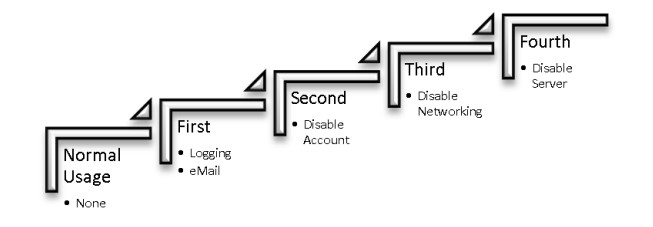
\includegraphics[width = 14cm]{images/responses.jpg}
  \caption{ Gradual responses to file changes according to thresholds set by the admin.}
  \label{fig:irradiances}
\end{figure}
\FloatBarrier

\noindent This mechanism allows you to set your response gradually, avoiding to shutdown all services at once and therefore avoiding to have a large recovery time once the system is restarted.\\
A proprietary solution called \textit{EventSentry} offers this file integrity monitoring service, letting the user deploy a honeypot that monitors files of interest via GUI.

\subsubsection{Software Diversification}
Studies prove that one of the keys for the success of malware attacks is that attackers rely on the so-called "software monoculture". In other words, it is much more likely that an attack is successful when the software implementation of the victim's system or infrastructure is easy to guess.\\
A \textit{system call} is the way for a computer program to interact with the kernel of the operating system on which it is executed.\\
Two sets of system calls (well-known ones and hidden ones) can detect attacks if you let the trusted nodes only use the hidden ones, that are less likely to be guessed. Any traffic on the network that relies on the interface of well-known system calls is to be considered as malicious.\\
This solution allows you to let malware run freely and without any risk to the assets you want to defend. Thus, you can study the behavior of the malware and gather more information about it.\\
A drawback of this approach is that the malware attack could utilize the code already present in allowed operations.

%\subsubsection{Hybrid Honeypot: Low interaction + High interaction}
%\textcolor{red}{This honeypot framework got built for the IoT world, observing the vulnerabilities of IoT devices. It provides both a high interaction honeypot that simulates the services available in the system making them seem real and therefore very appealing for attackers and a low interaction honeypot with SSH service, to simulate the login procedure.}

\subsubsection{Machine Learning algorithms}
Literature is full of machine learning-based approaches regarding malware detection. They all use some kind of malware classifier whose purpose is to distinguish between malicious and benign software, with a certain degree of confidence. Here the system exposes some fake service and learns how to defend itself thanks to a training period that exploits a training data set, called "EMBER" as described in the article "The Endgame Malware BEnchmark for Research" \cite{https://doi.org/10.48550/arxiv.1804.04637}, which provides 900.000 training samples.\\
A classification technique often adopted in malware detection is the Decision Tree Algorithm, that classifies them based on malware features and behavior.\\
When a malware is detected the honeypot gives some details to the admin, which is supposed to be a cybersecurity expert, who can validate or deny the classification, making the algorithm train even further.\\
As an example, ransomware always carry a message through which the user is warned that they should pay a ransom (often asked in untraceable currency, like bitcoins) to get their data back from the malicious encryption.
This feature could be exploited for defense purposes because as soon as a malicious text is spotted through key words such as "pay", "blocked", etc you stop its spread.\\
This is clearly just an example since ransomware might not carry this message, or it might be encrypted. A high training period with a wide training data set could help you spot malware by features (e.g., some peculiar file size and code fragments) rather than by a ransom message.

\begin{figure}[h]
  \centering
  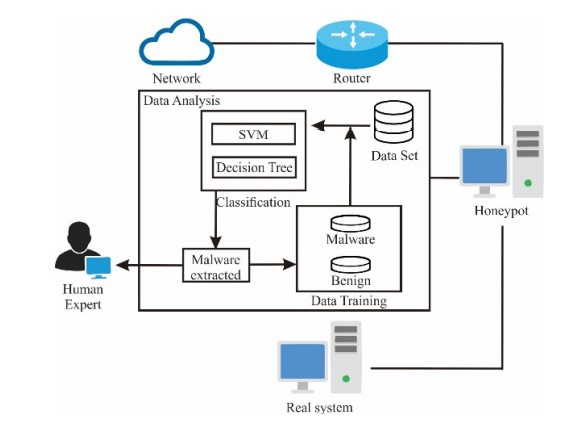
\includegraphics[width = 14cm]{images/machineLearning.jpg}
  \caption{ Example architecture of system with honeypot and machine learning.}
  \label{fig:irradiances}
\end{figure}
\FloatBarrier

\newpage


\section{Web application honeypot}
End-user applications are an intrinsic part of an IoT infrastructure. These help users in monitoring and controlling IoT devices from remote locations.\\
These applications transmit user commands to the cloud, and subsequently, to IoT-enabled devices connected to the network.\\
Mobile apps, web apps and desktop apps are the end-user applications found in an IoT infrastructure.\\
Web applications often get attacked causing a break into confidentiality and integrity of information using: 
% \begin{enumerate}
\begin{itemize}
    \item \textbf{SQL injection}: This is a type of attack granted by the fact that SQL doesn't check that whoever modifies the database has permission and a lack of input validation in web application can cause the success of this attack. The attacker can insert structured Query Language code as parts of final query string into a form that causes a web application to generate and send a query that works differently than the programmer intended;
    \item \textbf{Cross-site scripting (XSS)}: An XSS allows a cracker to insert or execute client-side code in order to collect, manipulate and redirect confidential information, or even view and modify data on servers or alter the dynamic behavior of web pages using any language ( example JavaScript, VBScript, Flash);
    \item \textbf{Remote file inclusion attacks(RFI)}: This attack is caused when an application builds a path given by the user via variable without checking its origin. The attacker modifies an user variable in the URI (example GET POST in PHP) perhaps adding maligns executable code, the web application downloads and runs the remote file;
    \item \textbf{Local file inclusion attacks(LFI)}: This attack is very similar to the previous one, in this case the application only executes files included in the server so the attacker inside the script tricks the application including another malignous script to execute.
% \end{enumerate}
\end{itemize}
In these cases a honeypot can be very useful.\\
The Honeypot can individuate the IP source of the attack, the purpose of the attack (if there was the intention of destroying or modifying the database etc), which methods are used by the attacker to capture data and what is the most attacked part of the database.\\
The Web application Honeypot must respond to the attacker in a best possible way to better deceive him/her.
\subsection{DShield Web Honeypot}
The idea of this Honeypot starts with DSHield, a firewall log correlation system used by the SANS institute to collect logs received by volunteers worldwide and analyze them providing which IPs are more dangerous, which port are more used for attacks etc etc.\\
The honeypot is a low-latency one that collects logs from web apps adding them to all the logs that already are sent to DShield, this logs contains the URL and header information  such as IP address, host, user agent, referring from all requests (even harmless ones) and, after being checked with expressions in \textit{config.txt} file, they are saved inside the logs folder of the honeypot and then posting it to the DShield database (this is done every 30 minutes).\\
The honeypot works in a simple manner: on the inside it contains a set of templates and a login system; when an attack takes place, the template is chosen checking inside the set if a suitable one is present (if there is no template , it returns a default web page), the honeypot sends the response to the attacker meanwhile the request is logged and sent to the DShield database.

\begin{figure}[h!]
  \centering
   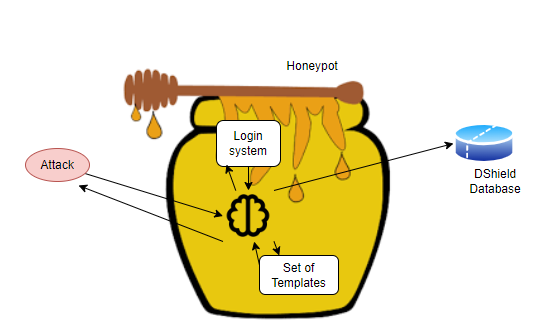
\includegraphics[width=10cm]{images/DSHoneypot.png}
   \caption{Structure of DShield honeypot}
  \label{fig:irradiances}
\end{figure}
\FloatBarrier


All of this idea can be download for free, this because all the logs are useful to the project. It is also used by home connection to collect data (as a peer to peer net "the more the better").

\subsection{Glastopf}
Glastopf is a very old Python web application low-interaction honeypot able to produce web applications vulnerable also to SQL injection. Glastopf manages to emulate vulnerability types, this allows us to manage multiple attacks of the same type until the attacker finds another fail in the web application or a new attack method.\\
Attackers will find the web service and try to attack the system, it is detected and gets logged by the honeypot that inserts all the information in the logs file (or database).\\
It has a good capability of logging based on the interaction that an attacker would have with the application but it shows some limitations: the front-end part is quite primary and attackers can easily recognize that this is not a real system and it only supports SQL injection, remote (RFI), and local file inclusion(LFI) vulnerabilities.

\subsection{Comparation between glastopf and DShield Honeypot}
In the paper of 2014 ,\textit{The Behavioural Study of Low Interaction Honeypots: DSHIELD and GLASTOPF in various Web Attacks}\cite{dshieldandGlastopf}, the interaction of these two honeypots with various attacks is put in comparison.\\
DShield and Galastpof have similar working techniques.
\begin{figure}[h!]
  \centering
   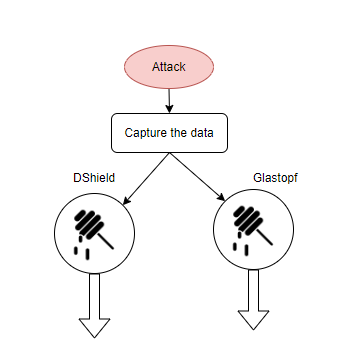
\includegraphics{images/workingtecniques.png}
   \caption{Flow of attack in DShield and Galastopf}
  \label{fig:irradiances}
\end{figure}
\FloatBarrier
DShield has a better ability to categorize the type of attack and by means of Apache server it is possible to extract a report. On the other hand, it is not easy to go through the logs and understand attacks easily.\\
Galastopf has logs that are easy to understand and they also capture the HTML information that is posted within the request, the response from the server and response code (\texttt{200 OK}) confirming that the attack was successful on the other way cannot categorize the SQL injection and XSS and the logs generated for Remote File Inclusion attacks were lesser compared to Dshield.\\

\subsection{SNARE and Tanner}
SNARE (Super Next generation Advanced Reactive honEypot) is a web application honeypot sensor attracting all sort of maliciousness from the Internet.\\
It pays attention to the web site,in fact has an inbuilt Cloner that, invoked before SNARE, clones all the web pages given as input, all the images on the web pages, scripts and action elements so that the clone looks as good as a real system.\\
SNARE needs TANNER to work. It is a remote data analysis and classification service to evaluate HTTP requests and composing the response then served by SNARE. TANNER uses multiple application vulnerability type emulation techniques when providing responses for SNARE, so it creates each time a new session for a new attack, each session tries to detect the attacker (if it is a tool, an user or a crawler), the location of the attack and shows through the TANNER UI for the administrator statistics regarding how many attacks of that kind have been found; after that, it emulates the response (via an emulator) and gives the attacker the response as the website would do.

\begin{figure}[h!]
  \centering
  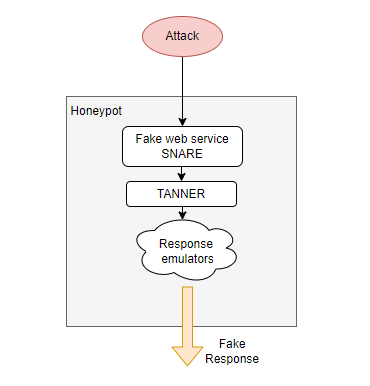
\includegraphics{images/DHP.png}
  \caption{Structure of SNARE and TANNER}
  \label{fig:irradiances}
\end{figure}
\FloatBarrier
\subsection{Solution of Honeypot with SNARE}

In the paper \textit{An Innovative Security Strategy using Reactive Web Application Honeypot}\cite{https://doi.org/10.48550/arxiv.2105.04773}, a solution for a web application honeypot which includes many emulators for very complex vulnerabilities is proposed. Its structure is the following manner:
\begin{enumerate}
    \item SNARE: It serves all the web pages on top of itself, becoming a server and hence monitoring all the HTTP events/flows throughout the application, similar to a real system;
    \item TANNER: It analyzes the requests made through SNARE after that it generates the responses dynamically;
    \item Database: for attack classifications;
    \item Docker: Docker is used to create containers for the emulators;
    The emulator creates a container for different custom images, executes the payload of the attacker, takes the credible result and deletes the container so that libraries are used inside a container and cannot damage the system, the honeypot remains secure;
    \item Emulation engine: every event on SNARE has to pass through all types of emulators: GET,POST and cookies emulators;
    \item PHP Sandbox (PHPOX): it returns emulation results for emulators like PHP object/code injection, XXE injection, and RFI;
    \item Base Emulator: it manages all the other emulators supporting multiple vulnerabilities and prepares the custom page for the injection;
    \item Template Injection Emulator: this emulator imitates the Template Injection vulnerability. The input payload is matched with the element in the database to identify the type of attack, then it is injected into the docker vulnerable custom template of that type and, after the execution, the final results are sent to SNARE;
    \item XML External Entity (XXE) Injection Emulator: same story of the Template injection Emulator. It emulates XML External Entity Injection vulnerability and Out of Band XXE Injection as well;
    \item PHP Object/Code Injection Emulator: it emulates the PHP Object Injection vulnerability. The injection results are sent to SNARE from PHP sandbox so the code is executed in PHP sandbox safely;
    \item Attacker/Crawler Detection: it allows to detect if the attacker is a crawler or a tool and tries to get the owner.
\end{enumerate}
\begin{figure}[h!]
  \centering
  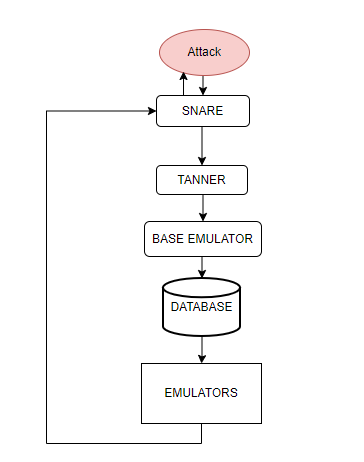
\includegraphics{images/solution.png}
  \caption{Structure of the honeypot}
  \label{fig:irradiances}
\end{figure}
\FloatBarrier

\section{Virtual Honeypot}
A virtual honeypot is a software that emulates a vulnerable system or network to attract intruders and study their behavior. It is easy to implement and unlike hardware-based, it can contain in a single Virtual machine multiple honeypots implemented for different purposes and since it is all emulated it does not allow infiltrations from the outside that can use the same virtual honeypot to attack the system, but because it is completely emulated, a skilled hacker can see the difference from the real system.
\subsection{A tool for virtual honeypot: Honeyd}
Honeyd is a small daemon that creates virtual hosts on a network. It creates low-interaction honeypots that emulate the service of a real OS.
It allows you to create multiple virtual honeypots (each with a different IP) by sharing the resources of the same server.\\
The server via TCP / IP protocol, based on the destination IP address, chooses which honeypot to serve.\\
It only supports TCP, UDP, and ICMP protocols.\\
Honeyd , as explained in the article \cite{Provos2003HoneydA} is designed for Unix systems and (as the other low-interaction honeypot) it has no OS installed, it has the advantage of running several different operating systems at the same time, each IP has his port to make the service listen and return different fake message returning them to the hacker, this fake message is generated by personality engine to make it look good and logical according to the template.\\
The template is a virtual machine where we can set which ports are open, which OS is running etc. each port can be set to be open with a script running on it to simulate the service.\\
\begin{figure}[h!]
\centering
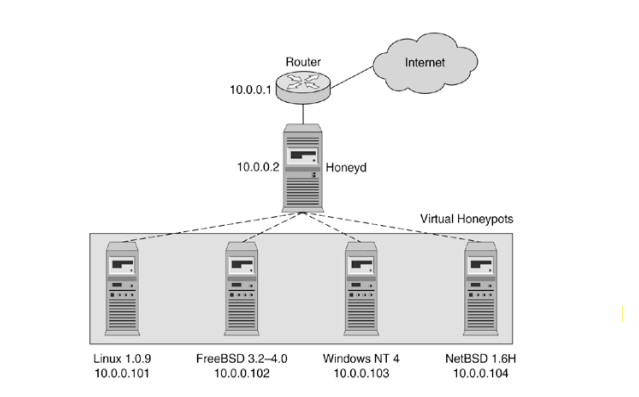
\includegraphics{images/honeyd1.png}
\caption{Structure of the honeyd}
\label{fig:irradiances}
\end{figure}
\FloatBarrier
The file Honeyd.conf contains the configuration for the virtual network .\\
Once the template is fixed we can set the IP addresses, at the end we create a network that seems real to the attacker.\\

As soon as a packet arrives, the dispatcher checks that the IP is valid in the configuration file, in the absence of the IP a default model is sent back.
\begin{figure}[h!]
\centering
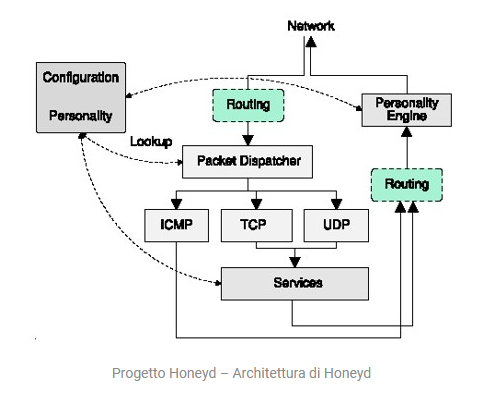
\includegraphics{images/honeyd.png}
\caption{Implementation of honeyd}
\label{fig:irradiances}
\end{figure}
\FloatBarrier
Upon receipt of a request, the framework checks whether the packet concerns an already established connection and in this case forwards it to the corresponding service, otherwise a new process is created for its execution. In addition to local services, a connection redirection mechanism is supported through which it is possible to route a service request to a real system.
The personality engine and configuration engine work together to decide the protocol for transferring according to the configuration (transport and link layer), so before returning the packets to the network, the personality engine modifies the headers to make them compatible with the stack used in the machine's SO.\\
Since attackers often use tools to scan the network and know the operating system running on the system, by default Honeyd uses Nmap's fingerprinting database as a reference for TCP headers and Xprobe's for ICMP headers. In this way, he tries to deceive the attackers with their weapons.
Since both the DOS Honeypot and Malware Honeypot works with TCP/IP protocol, we think it should be a good idea to run this daemon inside one Raspberry Pi and generate both the honeypots in virtual.
Honeyd is a very interesting low interaction honeypot but its problem is its age, apparently, the project is outdated and nobody seems to upgrade it.\\
Another problem given by age is that hacker tools are evolving over time so identifying this honeypot is not so hard.\\
Now with a basic scan, it is possible to find which ports are open, connect to them and as soon as the connection is established the hacker (based on the response the honeyd provides) understands quickly that something is wrong and aborts the attack.

\section{DoS attack}

A DoS attack takes place when a client is used by the attacker to flood with TCP and UDP packets one target server overriding the resources of a system so that it cannot respond to service requests of legitimate users. This causes bandwidth saturation and the exhaustion of computing resources, even leading to a server crash.\\
A DDoS attack takes place when multiple systems target a single system with a DoS attack, more difficult to be tracked because the attack is launched by various positions.\\
Citing an example, one major use of IoT is home automation
systems. If an attacker attacks the main server of such a
system with a DoS attack, the whole system tends to shut
down and any appliance within the whole house (sometimes
even door locks) is made inaccessible. This small example
shows the significance of security implementation in IoT.
In IoT-based networks, new devices that enter the
network are configured automatically due to their open nature.
This leaves such networks prone to a lot of attacks. The open
nature of IoT makes it relatively easy for spammers and
attackers to infiltrate IoT networks and launch DoS attacks.

\subsection{Different type of Dos attack}
Unfortunately exist very different types of Dos attacks, based on the protocol that is used, if the aim is crash services or flood services. For example in a yo-yo attack, the attacker generates a flood of traffic until a cloud-hosted service scales outwards to handle the increase of traffic, then halts the attack, leaving the victim with over-provisioned resources. When the victim scales back down, the attack resumes, causing resources to scale back up again.
An example of a TCP attack is \textbf{SYN Flood Attack}. To better understand it we need a closer look at how TCP initializes a connection between a client and a server.

The algorithm used by TCP to establish and terminate a connection is called a three-way handshake.
The idea is that two parties want to agree on a set of parameters, which, in the case of opening a TCP connection, are the starting sequence numbers the two sides plan to use for their respective byte streams. In general, the parameters might be any facts that each side wants the other to know about. First, the client (the active participant) sends a segment to the server (the passive participant) stating the initial sequence number it plans to use (Flags = SYN, SequenceNum = x). The server then responds with a single segment that both acknowledges the client's sequence number (Flags = ACK, Ack = x + 1) and states its own beginning sequence number (Flags = SYN, SequenceNum = y). That is, both the SYN and ACK bits are set in the Flags field of this second message. Finally, the client responds with a third segment that acknowledges the server's sequence number (Flags = ACK, Ack = y + 1). The reason why each side acknowledges a sequence number that is one larger than the one sent is that the Acknowledgment field actually identifies the “next sequence number expected,” thereby implicitly acknowledging all earlier sequence numbers.
To better understand the step to establish the connection, please refer to the figure below.
\begin{figure}[h!]
\centering
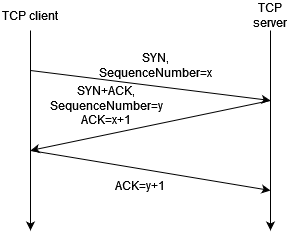
\includegraphics[width = 10cm]{images/TCP3wayHANDSHAKE.drawio.png}
\caption{TCP handshake protocol}
\label{fig:TCP}
\end{figure}
\FloatBarrier
\noindent

An attacker that wants to establish a \textbf{SYN Flood Attack} creates a bot that creates thousands of first segments in the 3-way handshake protocol. Then when the server replies with the SYN-ACK packet, the bot client never reply to it to make thousands of incomplete request of connection to the server to slow down it. Please refer to the picture below.

\begin{figure}[h!]
\centering
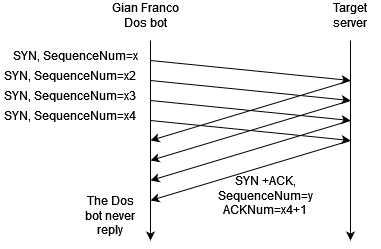
\includegraphics[width = 10cm]{images/DosSYNFloodAttack.drawio.png}
\caption{TCP SYN flood attack}
\label{fig:TCPDos}
\end{figure}
\FloatBarrier
\noindent
Now, the following question is, could we use honeypots to avoid this type of TCP attack?
According to what we found on the internet, to protect our servers from the \textbf{SYN Flood Attack}, is better to:
\begin{itemize}
\item Installing an IPS to detect anomalous traffic patterns;
\item configure the onsite firewall for SYN Attack Thresholds and SYN Flood protection;
\item Installing up-to-date networking equipment that has rate-limiting capabilities.
\end{itemize}
So honeypots are not useful to prevent that.
\section{MITM attack and honeypots}
%Does a honeypot could help in the protection from the MITM attack?
%First we need to explain what is a MITM attack. 
In a server-client architecture, a MITM attack takes place when the attacker is inserted inside the communication between client and server. Let's make an example of possible situation that could occur, and a proposal of honeypot that could resolve it. \\
The normal procedure to avoid MITM attack is to encrypt and decrypt data between client and server. The main steps are:
\begin{enumerate}
    \item \textbf{Use asymmetrical encryption}. First we use an asymmetric algorithm to allow us to send in a secure way the symmetric key that will be used in the future;
    \item \textbf{Use symmetric encryption}. Now that the symmetric key is shard between the server and the client, the data are sent normally between the ends points and not anyone in the middle can understand them.  
\end{enumerate}

\noindent What if the first step fails? As an example,our IoT server for example could use a weak RSA algorithm, based on 16 bit key. Our men in the middle could manage to find the private key of the server and decrypt the symmetric key that will be used in the second step, like shown in the figure below.

\begin{figure}[h!]
  \centering
  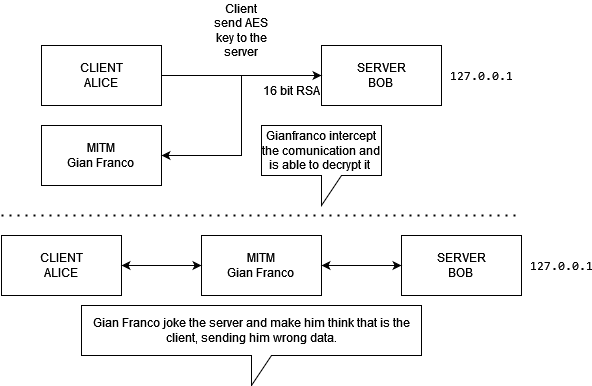
\includegraphics[width = 15cm]{images/MITMExampleAttack.drawio.png}
  \caption{An example on MITM attack}
  \label{fig:4period}
\end{figure}
\FloatBarrier

\noindent How can our system understand that it is speaking to a MITM and not to the client? Our honeypot would intervene right here.\\
For example, it could first check if the wrong data sent by the MITM makes sense or not. Then it could check if the data of the fake sensor makes sense with respect to a set of data collected from the real sensor in the precedent days. If the honeypot recognizes that a man in the middle is present, it could collect data about the hacker and see what information they are trying to capture, which attacks he/she is trying to inject in to the network, studying  the methodology used by hackers. Moreover, a honeypot AP could (at least temporarily) keep the hacker engaged and alert the administrator so that the actual network can be safeguarded.then close the collection. If no violation is detected, the honeypot sends the data to the real server. A possible implementation is show in the figure below.

\begin{figure}[h!]
  \centering
  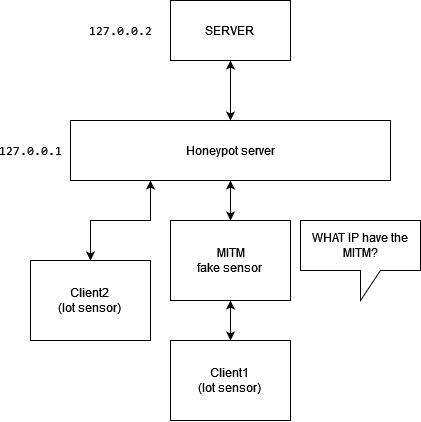
\includegraphics[width = 15cm]{images/MITMHONEYPOT.drawio.png}
  \caption{A possible system structure for the MITM honeypot.}
  \label{fig:5period}
\end{figure}
\FloatBarrier

\section{FAKEHONEYMITM (MITM attacks and honeypots)}
Regarding the MITM attack, we have another possible idea to implement. As we know, a man in the middle tries to place himself between the sensors of the IoT cluster and the servers inside the network. He need to intercept the message from the sensors to the servers and viceversa. But what if the sensor is not real but is a honeypot? For example our cluster could expose a connection between 2 honeypots, the first one is a fake server, the second one is a fake sensor. But why an attacker have to choose this connection for him malicious purpose? Well, this link could work with a weak encryption to seems like a vulnerability of our network. When the MITM manage to put itself between the fake connection, our honeypots could collect data on the activity of the hacker. To better understand this idea, please refer to the figure (\textcolor{blue}{\ref{fig:MITMFakeSensor}})

\begin{figure}[h!]
  \centering
  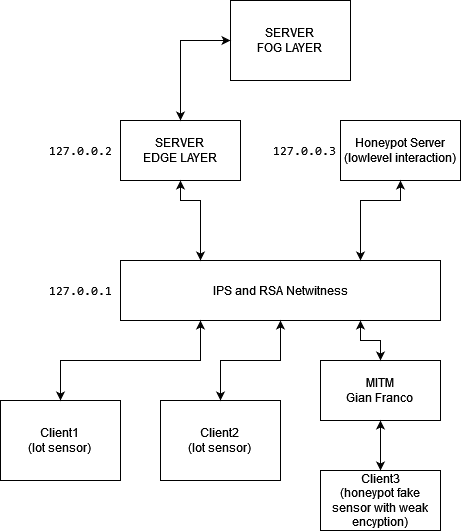
\includegraphics[width = 10cm]{images/MITMFakeSensor.drawio.png}
  \caption{A possible structure for the fake sensor honeypot and MITM}
  \label{fig:MITMFakeSensor}
\end{figure}
\FloatBarrier



\section{Eavesdropping Attack and Countermeasures}
\subsection{Eavesdropping Attack}
In eavesdrop attack the network is sniffed in order to retrieve information transmitted through the network itself; the process can be classified as passive or active depending on the existence of an interaction of the attacker on the network. Specifically, a passive attack is performed just analyzing packets of information on the eavesdropped network channel, while an active attack is performed requesting directly to the channel information the attacker wants to retrieve.\\
To counteract eavesdropping phenomena on a network several possibilities are present, always keeping in mind that the desired objective is to maintain secrecy of transmitted information.

\subsection{Encrypting the channel}
The most straightforward method to secure a channel communication is to encrypt the transmitted data, in this way even if the channel is sniffed data are secured (assuming a safe key maintenance and management). This solution is great for networks/clusters of powerful computers or for application that require not sending too many data, otherwise the risk is to spent most of the time computing cryptographic algorithms instead of computing for the cluster purpose. Mitigations could be the design of specific hardware to accelerate those computations; this implies that the applicability of this solution is impossible for most of the cheap low-cost low-power IoT-cluster applications.

\subsection{Physical Countermeasures}
\subsubsection{Intelligent Reflecting Surface}
A solution in proposed in the article \textit{"Eavesdropping with Intelligent Reflective Surfaces: Threats and Defense Strategies"}\cite{https://doi.org/10.48550/arxiv.2108.00149} will enhance the point-to-point communication between the sender and the receiver making it impossible for the attacker to read the channel. This result is obtained exploiting properties of reflecting surfaces able to dynamically re-adapt and focus the connection to one specific point. Specifically, the channel for the attacker is worsen to a level of binary gibberish securing the information in the meanwhile.
\subsubsection{Channel Capacity and Information Freshness}
Other techniques are related to evaluating the capacity of the two receiving nodes (the actual receiver and the eavesdropper), CD and CE, and trying to set a network transmission protocol to make the eavesdropper unable to receive the data up to a given secrecy level RS as perfectly desctibed in the paper \textit{"Relay Selection for Wireless Communications Against Eavesdropping: A Security-Reliability Tradeoff Perspective"} \cite{Zou_2016}\\
For systems in which the useful information is related to the freshness of the obtained data and the only secrecy that matters is the one aimed in protecting the newest data (we can imagine systems analyzing the position of cars on the road) other metrics have been developed ("secrecy age" and "secrecy age outage") as the article \textit{"Secure Status Updates under Eavesdropping: Age of Information-based Physical Layer Security Metrics"}\cite{https://doi.org/10.48550/arxiv.2002.07340}.

\subsection{Impulsive Statistical Fingerprinting}
This method is trying to move in the direction of cryptographic methods, without the usage of standard cryptographic algorithms, The point of this technique is to remove information that make the data understandable before transmitting it. The method relies on the exchange of fingerprints (e.g. time-stamps) between the source node and the destination node. These fingerprints are then used to compute statistics using some algorithms (final results will be mean, std deviation, other order momentum, and so on..) and to manipulate data before transmitting those by manipulations like removing the mean, whiten the data by dividing it by the std-deviation, etc. This method is suitable for the usage on low-performance IoT-clusters; on the other hand it is not mathematically secure: the method relies on the fact that an attacker will not be able to get a sufficient number of fingerprints to then be able to retrieve information on the transmitted data.

\subsection{Active Eavesdropping - ML approach}
All of previous remedies are for passive eavesdropping. For active eavesdropping there is the necessity to treat requests through the channel. Common possibility is to reduce the permission of requests from class of nodes. Another approach is to exploit ML to perform anomaly-detection classifying series of actions as normal or anomaly. Algorithms suitable for IoT-class devices can be random trees (random forests in the case of parallel execution on all the IoT-cluster), or comparison based like K-nearest neighbors, or linear methods like logistic regression or Perceptron based approach; in the case of NN (Neural Network) this must be conceived specifically for the device it will be deployed considering HW resources and computation capabilities. In all these cases features can be collected from the normal network traffic in a protected environment and then used to in the training procedure.

\subsection{Possible Honeypots}
Honeypots can work together with the identification procedure provided by previous techniques; as an example an useful honeypot approach could be in jamming the channel once the attacker is identified. Or keeping an unprotected (less protected) channel the attacker will try to get access to first and that is sending fake, but coherent, data.

\section{Password Attack and countermeasures}
\subsection{List of counteracts and considerations}
\begin{itemize}
  \item Limit the number of attempts and track the requester;
  \item Since an attacker will try first to use common passwords maybe related to personal accessible info, a possibility is to keep a blacklist of possible passwords created from those personal info (that we also know..) and block the attacker attempts immediately;
  \item A honeypot approach could be, in the case of previous condition, to give access to a fake shell in order to evaluate requests from the attacker, while taking countermeasures.
\end{itemize}

